% begin module function-piecewise
\begin{frame}
\frametitle{Piecewise Defined Functions}
\begin{definition}[Piecewise Defined Function]
A piecewise defined function is a function that is defined by different algebraic formulas on different subsets of its domain.
\end{definition}
\uncover<2->{
\begin{example}
\begin{columns}[t]
\column{.4\textwidth}
\psset{xunit=0.8cm, yunit=0.8cm}
\begin{pspicture}(-5, -5)(5,5) 
\psframe*[linecolor=white](-5,-5)(5,5) 
\psaxes[ticks=none, labels=none]{<->}(0,0)(-3,-1.5)(3,1.5)\tiny
\psLabelsWithOnes{3}{1.5}
\psline[linecolor=red](-3, -1)(0,-1)
\psline[linecolor=red](3, 1)(0,1)
\psHollowDot{0}{-1}
\psFullDot{0}{1}
\end{pspicture} 
%\ 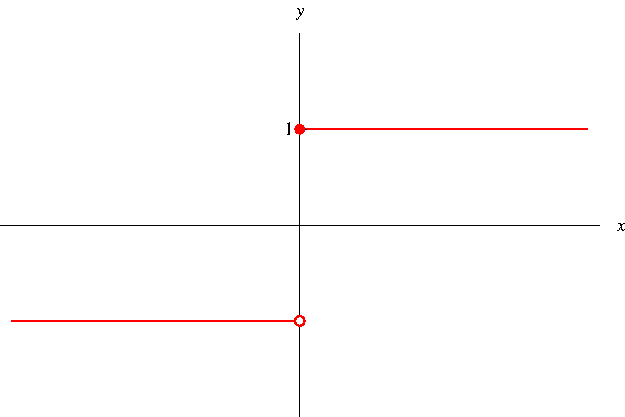
\includegraphics[height=3.5cm]{precalculus/pictures/01-01-piecewise.pdf}
\column{.5\textwidth}
\[
f(x) = \left\{ \begin{array}{rcc}
1 & \textrm{ if } & x \geq 0 \\
-1 & \textrm{ if } & x < 0 
\end{array}\right. 
\]

The filled red circle means $(0,1)$ is on the curve.  

The open circle means $(0, -1)$ is not on the curve.
\end{columns}
\end{example}
}
\end{frame}
% end module function-piecewise
